\documentclass[aspectratio=169,11pt]{beamer}

\usetheme{Madrid}
\usecolortheme{default}

\usepackage{amsmath,amssymb,bm}
\usepackage{graphicx}
\usepackage{booktabs}
\usepackage{array}
\usepackage{xcolor}

\definecolor{deepblue}{RGB}{24,64,112}
\definecolor{softblue}{RGB}{230,240,252}
\definecolor{softgreen}{RGB}{232,247,238}
\definecolor{softorange}{RGB}{255,242,225}
\definecolor{darkgreen}{RGB}{34,112,72}
\definecolor{darkorange}{RGB}{180,96,32}

\setbeamercolor{frametitle}{fg=white,bg=deepblue}
\setbeamercolor{title}{fg=deepblue}
\setbeamercolor{block title}{fg=white,bg=deepblue}
\setbeamercolor{block body}{bg=softblue}
\setbeamercolor{alerted text}{fg=darkorange}
\setbeamertemplate{navigation symbols}{}
\setbeamertemplate{footline}[frame number]

\newcommand{\whatwhy}[2]{%
\begin{columns}[T,onlytextwidth]
  \begin{column}{0.48\textwidth}
    \begin{block}{What we do}
      #1
    \end{block}
  \end{column}
  \begin{column}{0.48\textwidth}
    \begin{block}{Why we do it}
      #2
    \end{block}
  \end{column}
\end{columns}
}

\newcommand{\smallgap}{\vspace{0.45em}}

\title[Step-by-Step SCS Design]{Step-by-Step Design of a Score-Only Sparse Electrode Attack on EEG Recognition}
\author{Duc Trong Minh Hoang}
\institute{INRS}
\date{}

\begin{document}

% ------------------------------------------------------------
\begin{frame}
  \titlepage
  \vspace{-1em}
  \begin{center}
    \small
    Goal of this version: assume no adversarial-attack background and explain each design step before the math.
  \end{center}
\end{frame}

% ------------------------------------------------------------
\begin{frame}{What The Audience Should Understand By The End}
\begin{enumerate}
  \item What an EEG recognition model does under normal use.
  \item What an adversarial attack means in this setting.
  \item Why EEG needs a different sparsity idea than images.
  \item Why the attack is score-only, channel-sparse, and EEG-band constrained.
  \item How sparse-channel search (SCS) builds the perturbation step by step.
  \item What the result \(k^\star\) means and why it is useful for security evaluation.
\end{enumerate}
\end{frame}

% ------------------------------------------------------------
\begin{frame}{One-Sentence Summary Before Details}
\begin{block}{The problem}
Can a deployed EEG identity recognizer be fooled when an attacker can only query output scores and perturb a few complete electrode traces?
\end{block}

\begin{block}{The design}
SCS first finds high-leverage EEG channels, then tunes small EEG-band waveforms on those channels until the model's predicted identity changes.
\end{block}

\begin{block}{The measurement}
\(k^\star\) asks: how many complete electrode traces were needed before the first successful flip?
\end{block}
\end{frame}

% ------------------------------------------------------------
\begin{frame}{First: What Is EEG Recognition?}
\begin{columns}[T,onlytextwidth]
  \begin{column}{0.48\textwidth}
    \begin{block}{Input}
      An EEG trial is a multichannel time series:
      \[
      \mathbf{X}\in\mathbb{R}^{C\times T}
      \]
      \(C\): electrodes. \quad \(T\): time samples.
    \end{block}
  \end{column}
  \begin{column}{0.48\textwidth}
    \begin{block}{Output}
      The recognizer gives one score per enrolled subject:
      \[
      f(\mathbf{X})=(f_1(\mathbf{X}),\ldots,f_K(\mathbf{X})).
      \]
      The predicted identity is the highest-score subject:
      \[
      \hat{y}(\mathbf{X})=\arg\max_j f_j(\mathbf{X}).
      \]
    \end{block}
  \end{column}
\end{columns}

\smallgap
\begin{center}
\small Clean recognition asks: does the system identify the subject correctly when the signal is not manipulated?
\end{center}
\end{frame}

% ------------------------------------------------------------
\begin{frame}{Security Asks A Different Question}
\begin{columns}[T,onlytextwidth]
  \begin{column}{0.48\textwidth}
    \begin{block}{Normal evaluation}
      \begin{itemize}
        \item Input: clean EEG trial.
        \item Output: predicted subject identity.
        \item Metrics: accuracy and biometric EER.
      \end{itemize}
    \end{block}
  \end{column}
  \begin{column}{0.48\textwidth}
    \begin{block}{Adversarial evaluation}
      \begin{itemize}
        \item Input: slightly modified EEG trial.
        \item Output: does the predicted identity change?
        \item Metrics: attack success and required channel budget.
      \end{itemize}
    \end{block}
  \end{column}
\end{columns}

\smallgap
\begin{center}
\alert{A model can be accurate on clean EEG but still fragile to carefully chosen input changes.}
\end{center}
\end{frame}

% ------------------------------------------------------------
\begin{frame}{What Is An Adversarial Attack?}
\begin{block}{Plain-language definition}
An adversarial attack adds a small, intentional perturbation to the input so that the model makes a wrong decision.
\end{block}

\begin{block}{In our EEG setting}
\[
\mathbf{X}^{adv}=\mathbf{X}+\mathbf{E}
\]
where \(\mathbf{X}\) is the clean EEG trial and \(\mathbf{E}\) is the perturbation.
\end{block}

\begin{block}{Success condition}
\[
\hat{y}(\mathbf{X}+\mathbf{E})\neq \hat{y}(\mathbf{X})
\]
The attack is non-targeted: any wrong identity is enough.
\end{block}
\end{frame}

% ------------------------------------------------------------
\begin{frame}{Why EEG Is Not Just An Image Attack}
\begin{columns}[T,onlytextwidth]
  \begin{column}{0.48\textwidth}
    \begin{block}{Image intuition}
      Sparse often means changing a few pixels.

      \smallgap
      A pixel is a natural visible unit in an image.
    \end{block}
  \end{column}
  \begin{column}{0.48\textwidth}
    \begin{block}{EEG intuition}
      EEG is measured by electrodes.

      \smallgap
      A complete electrode trace is a natural acquisition unit.
    \end{block}
  \end{column}
\end{columns}

\smallgap
\begin{center}
\alert{So the sparse unit should be a channel, not an isolated time sample.}
\end{center}
\end{frame}

% ------------------------------------------------------------
\begin{frame}{Threat Model: What The Attacker Can And Cannot See}
\whatwhy{
\begin{itemize}
  \item The attacker can submit EEG trials.
  \item The attacker observes output scores.
  \item No model weights.
  \item No gradients.
  \item No training data.
\end{itemize}
}{
\begin{itemize}
  \item Deployed systems usually hide internals.
  \item Scores are a realistic interface for many recognition systems.
  \item This makes the attack black-box and score-only.
\end{itemize}
}
\end{frame}

% ------------------------------------------------------------
\begin{frame}{Attack Surface: What The Attacker Controls}
\whatwhy{
\begin{itemize}
  \item The attacker perturbs only a few complete electrode traces.
  \item The classifier itself is unchanged.
  \item The subject's brain activity is not changed.
  \item The manipulation is modeled at the acquisition or digital input level.
\end{itemize}
}{
\begin{itemize}
  \item Complete electrode traces correspond to sensor paths.
  \item A few-channel attack is easier to interpret than dense noise.
  \item The channel count becomes a hardware-relevant security cost.
\end{itemize}
}
\end{frame}

% ------------------------------------------------------------
\begin{frame}{Constraint 1: Sparse Complete-Channel Control}
\begin{block}{Perturbation matrix}
\[
\mathbf{E}\in\mathbb{R}^{C\times T}
\]
Each row is one electrode trace.
\end{block}

\begin{block}{Active channel set}
\[
\mathcal{S}(\mathbf{E})=\{c:\|\mathbf{E}_{c,:}\|_2>0\}
\]
\end{block}

\begin{block}{Channel sparsity cost}
\[
\|\mathbf{E}\|_{\mathrm{ch},0}=|\mathcal{S}(\mathbf{E})|
\]
This counts how many complete electrode traces are changed.
\end{block}
\end{frame}

% ------------------------------------------------------------
\begin{frame}{Constraint 2: Bounded Amplitude}
\whatwhy{
\begin{itemize}
  \item The perturbation cannot be arbitrarily large.
  \item We cap the maximum sample value:
  \[
  \|\mathbf{E}\|_\infty \leq \eta\|\mathbf{X}\|_\infty .
  \]
  \item In the main experiments, \(\eta=10\%\).
\end{itemize}
}{
\begin{itemize}
  \item Without an amplitude cap, flipping the classifier is too easy.
  \item The cap makes perturbations comparable across trials.
  \item It keeps the attack closer to plausible signal injection.
\end{itemize}
}
\end{frame}

% ------------------------------------------------------------
\begin{frame}{Constraint 3: EEG-Band Waveforms}
\whatwhy{
\begin{itemize}
  \item On each selected channel, SCS injects a smooth waveform.
  \item The waveform is built from oscillatory basis atoms:
  \[
  \delta_c(t)=\sum_i a_{c,i}\phi_i(t).
  \]
  \item The atoms cover EEG-relevant frequencies.
\end{itemize}
}{
\begin{itemize}
  \item Arbitrary noise can look like an artifact.
  \item EEG recognition uses frequency structure.
  \item A basis reduces the search from all samples to a few coefficients.
\end{itemize}
}
\end{frame}

% ------------------------------------------------------------
\begin{frame}{How Do We Know The Attack Is Close To Success?}
\begin{block}{Clean winner}
\[
y_0=\hat{y}(\mathbf{X})
\]
\end{block}

\begin{block}{Decision margin}
\[
M(\mathbf{X},y_0)=f_{y_0}(\mathbf{X})-\max_{j\neq y_0}f_j(\mathbf{X})
\]
\end{block}

\begin{block}{Interpretation}
\begin{itemize}
  \item \(M>0\): the clean winner is still ahead.
  \item \(M=0\): another identity ties the clean winner.
  \item \(M<0\): some other identity has passed the clean winner, so the attack succeeds.
\end{itemize}
\end{block}
\end{frame}

% ------------------------------------------------------------
\begin{frame}{The Ideal Problem In One Slide}
\begin{block}{Goal}
Find the smallest number of electrode traces whose bounded perturbation flips the identity.
\end{block}

\[
\begin{aligned}
\min_{\mathbf{E}} \quad
& \|\mathbf{E}\|_{\mathrm{ch},0}\\
\mathrm{s.t.}\quad
& M(\mathbf{X}+\mathbf{E},y_0)<0,\\
& \|\mathbf{E}\|_\infty\leq \eta\|\mathbf{X}\|_\infty.
\end{aligned}
\]

\begin{center}
\small This is the clean design target. SCS is the practical black-box method we use to search for a solution.
\end{center}
\end{frame}

% ------------------------------------------------------------
\begin{frame}{Why The Ideal Problem Is Hard}
\begin{enumerate}
  \item \textbf{Channel choice is discrete.} We must choose which subset of electrodes to touch.
  \item \textbf{Waveform choice is continuous.} After choosing channels, we must tune waveform coefficients.
  \item \textbf{The model is black-box.} We cannot compute gradients from the model internals.
  \item \textbf{The query budget is finite.} We cannot try every channel subset and every waveform.
\end{enumerate}

\smallgap
\begin{center}
\alert{This is why the algorithm has two pieces: channel search plus waveform refinement.}
\end{center}
\end{frame}

% ------------------------------------------------------------
\begin{frame}{Design Overview: SCS}
\begin{block}{Sparse-Channel Search}
\[
\text{clean EEG}
\rightarrow
\text{probe channels}
\rightarrow
\text{select channel}
\rightarrow
\text{refine waveform}
\rightarrow
\text{check success}
\]
\end{block}

\begin{block}{Why "hybrid"?}
It combines a discrete search over electrode channels with continuous optimization of waveform coefficients.
\end{block}

\begin{block}{Why repeat?}
We want the first channel budget that succeeds, not only the final attack at the largest budget.
\end{block}
\end{frame}

% ------------------------------------------------------------
\begin{frame}{Step 0: Start From A Clean-Correct Trial}
\whatwhy{
\begin{itemize}
  \item Pick a validation trial that the recognizer classifies correctly.
  \item Record its clean predicted identity \(y_0\).
  \item Compute the clean margin.
\end{itemize}
}{
\begin{itemize}
  \item If the model is already wrong, attack success is meaningless.
  \item Starting from \(y_0\) lets us attack without needing the true label at test time.
  \item The margin tells us how far the decision is from flipping.
\end{itemize}
}
\end{frame}

% ------------------------------------------------------------
\begin{frame}{Step 1: Build The EEG Waveform Basis}
\whatwhy{
\begin{itemize}
  \item Create smooth basis atoms \(\phi_i(t)\).
  \item Use tapered sinusoids and smooth residual atoms.
  \item Express each injected trace as coefficients times basis atoms.
\end{itemize}
}{
\begin{itemize}
  \item The basis makes the perturbation EEG-like by construction.
  \item It avoids searching over every time sample independently.
  \item It gives SPSA a smaller coefficient vector to optimize.
\end{itemize}
}
\end{frame}

% ------------------------------------------------------------
\begin{frame}{Step 2: Probe Candidate Channels Cheaply}
\whatwhy{
\begin{itemize}
  \item For each unused channel \(c\), try a few small random probe waveforms.
  \item Query the model scores.
  \item Measure how much the decision margin decreases.
\end{itemize}
}{
\begin{itemize}
  \item We need to know which channels have high leverage.
  \item Full optimization for every possible channel would be expensive.
  \item Cheap probes give a fast first estimate.
\end{itemize}
}
\end{frame}

% ------------------------------------------------------------
\begin{frame}{Step 3: Select The Most Useful Channel}
\whatwhy{
\begin{itemize}
  \item Add the candidate channel that gives the lowest probed margin.
  \item The selected set grows one channel at a time:
  \[
  \mathcal{S}_0=\varnothing,\quad
  \mathcal{S}_{k}=\mathcal{S}_{k-1}\cup\{c_k\}.
  \]
\end{itemize}
}{
\begin{itemize}
  \item Exhaustive subset search is combinatorial.
  \item Greedy selection gives a practical low-query approximation.
  \item One-channel-at-a-time growth lets us measure first success.
\end{itemize}
}
\end{frame}

% ------------------------------------------------------------
\begin{frame}{Step 4: Refine The Waveform On Selected Channels}
\whatwhy{
\begin{itemize}
  \item Keep the selected channel set fixed.
  \item Optimize the waveform coefficients on that set.
  \item Use SPSA, a gradient-free optimizer.
\end{itemize}
}{
\begin{itemize}
  \item The attacker only sees scores, so standard backpropagation is unavailable.
  \item SPSA estimates a useful update direction from score differences.
  \item It uses only two score queries per random direction.
\end{itemize}
}
\end{frame}

% ------------------------------------------------------------
\begin{frame}{SPSA In Plain Language}
\begin{enumerate}
  \item Randomly nudge all active waveform coefficients upward or downward.
  \item Query the model on the plus version and the minus version.
  \item If one direction lowers the margin, move coefficients in that direction.
  \item Clip or rescale the perturbation so the amplitude cap still holds.
  \item Repeat until the query budget is used or the decision flips.
\end{enumerate}

\smallgap
\begin{center}
\small SPSA is the black-box replacement for "take a gradient step."
\end{center}
\end{frame}

% ------------------------------------------------------------
\begin{frame}{Step 5: Check Whether The Attack Succeeded}
\whatwhy{
\begin{itemize}
  \item After refinement, compute the margin:
  \[
  M(\mathbf{X}+\mathbf{E},y_0).
  \]
  \item If it is negative, stop.
  \item Record the current channel count as \(k^\star\).
\end{itemize}
}{
\begin{itemize}
  \item The first successful channel count is the security measurement.
  \item A small \(k^\star\) means only a few electrode traces were enough.
  \item This is easier to interpret than only reporting final ASR.
\end{itemize}
}
\end{frame}

% ------------------------------------------------------------
\begin{frame}{SCS Algorithm: Slow Version For A Talk}
\begin{enumerate}
  \item Start with no attacked channels.
  \item For channel budget \(k=1,2,\ldots,B\):
  \item Probe each unused channel with small EEG-band waveforms.
  \item Add the channel that most reduces the decision margin.
  \item Refine waveform coefficients on all selected channels using SPSA.
  \item Enforce the amplitude cap after refinement.
  \item If the margin is negative, return success and \(k^\star=k\).
  \item If no budget succeeds, report failure within the tested budget.
\end{enumerate}
\end{frame}

% ------------------------------------------------------------
\begin{frame}{What SCS Is And Is Not}
\begin{columns}[T,onlytextwidth]
  \begin{column}{0.48\textwidth}
    \begin{block}{It is}
      \begin{itemize}
        \item A score-only attack method.
        \item A sparse complete-electrode control test.
        \item A way to measure channel-level fragility.
        \item A practical heuristic for a hard optimization problem.
      \end{itemize}
    \end{block}
  \end{column}
  \begin{column}{0.48\textwidth}
    \begin{block}{It is not}
      \begin{itemize}
        \item A new clean EEG classifier.
        \item A proof of the globally smallest perturbation.
        \item A hardware-in-the-loop injection experiment.
        \item A claim that every EEG task behaves the same way.
      \end{itemize}
    \end{block}
  \end{column}
\end{columns}
\end{frame}

% ------------------------------------------------------------
\begin{frame}{Evaluation Setup}
\begin{block}{Main study}
\begin{itemize}
  \item Dataset: HBN R1-L100 EEG release.
  \item Task: subject recognition.
  \item Train on passive-task windows; validate on active-task windows.
  \item Model: EEGConformer.
  \item Subject counts: 20, 35, 50, 75, 100, 122.
\end{itemize}
\end{block}

\begin{block}{Attack setting}
\begin{itemize}
  \item 64 EEG channels.
  \item Maximum channel budget \(B=12\).
  \item Peak-ratio cap: 10\%.
  \item Query budget: 45,000 score calls per trial.
\end{itemize}
\end{block}
\end{frame}

% ------------------------------------------------------------
\begin{frame}{Main Metrics}
\begin{block}{Clean metrics}
\begin{itemize}
  \item Validation accuracy: clean identification performance.
  \item EER: biometric verification quality.
\end{itemize}
\end{block}

\begin{block}{Attack metrics}
\begin{itemize}
  \item ASR: fraction of clean-correct trials flipped within the budget.
  \item Attacked accuracy: accuracy after applying the attack.
  \item Mean and median \(k^\star\): typical first-success channel count.
  \item \(K90\), \(K95\), \(K100\): channel counts needed to reach cumulative prefix ASR thresholds.
\end{itemize}
\end{block}
\end{frame}

% ------------------------------------------------------------
\begin{frame}{Result 1: HBN Subject-Count Sweep}
\begin{center}
\IfFileExists{Figure/hbn_scaling_dashboard.pdf}{%
  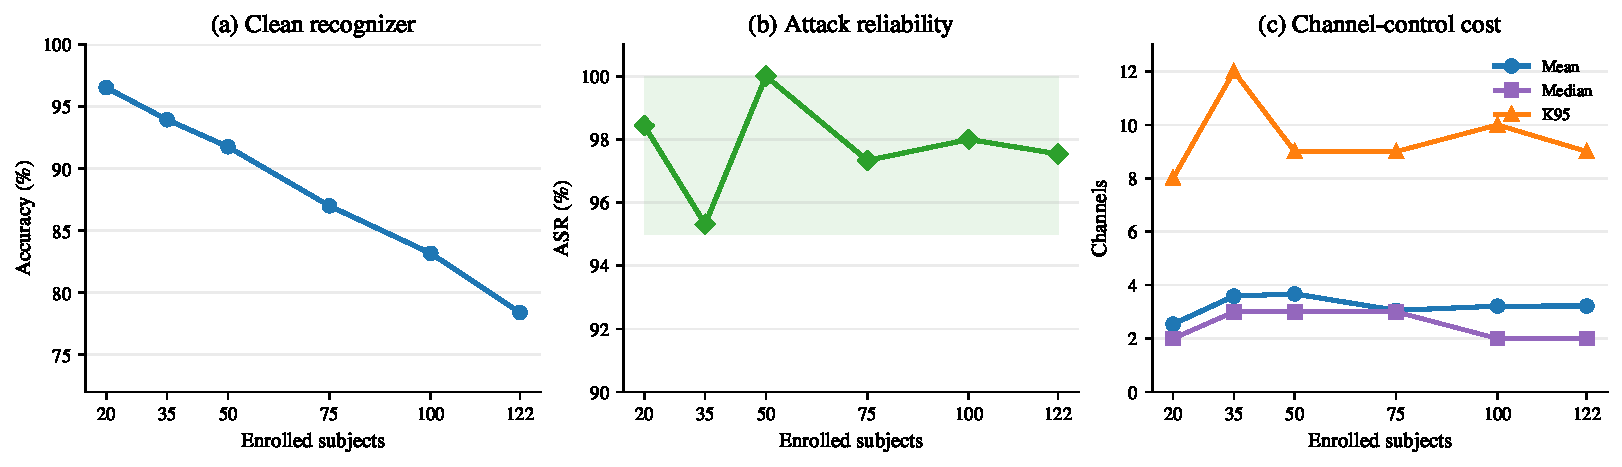
\includegraphics[width=0.95\textwidth]{Figure/hbn_scaling_dashboard.pdf}
}{%
  \fbox{\parbox{0.8\textwidth}{Figure/hbn_scaling_dashboard.pdf not found.}}
}
\end{center}
\vspace{-0.4em}
\begin{center}
\small Clean recognition gets harder as more subjects are enrolled, but SCS keeps high ASR and low first-success channel counts.
\end{center}
\end{frame}

% ------------------------------------------------------------
\begin{frame}{Result 1 In Words}
\begin{table}
\centering
\small
\begin{tabular}{rcccc}
\toprule
IDs & Clean acc. & EER & ASR & Mean \(k^\star\)\\
\midrule
20  & 96.55\% & 1.70\% & 98.44\% & 2.54\\
35  & 93.95\% & 1.85\% & 95.31\% & 3.59\\
50  & 91.77\% & 2.17\% & 100.00\% & 3.67\\
75  & 87.01\% & 2.96\% & 97.33\% & 3.05\\
100 & 83.18\% & 3.27\% & 98.00\% & 3.21\\
122 & 78.40\% & 4.10\% & 97.54\% & 3.22\\
\bottomrule
\end{tabular}
\end{table}

\begin{center}
\alert{Even for 122 enrolled subjects, the mean first-success count is only 3.22 channels.}
\end{center}
\end{frame}

% ------------------------------------------------------------
\begin{frame}{Result 2: Success Accumulates In The First Few Channels}
\begin{center}
\IfFileExists{Figure/hbn_prefix_success_curves.pdf}{%
  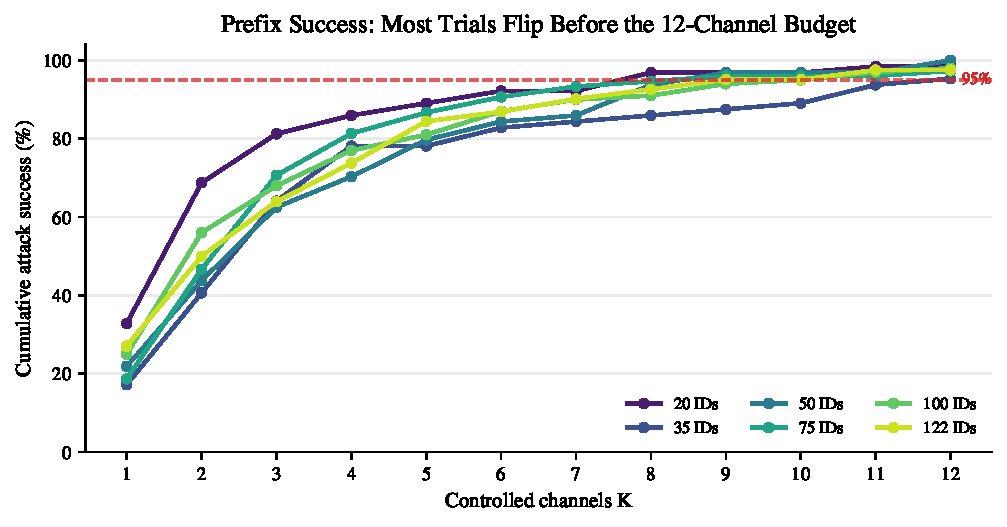
\includegraphics[width=0.82\textwidth]{Figure/hbn_prefix_success_curves.pdf}
}{%
  \fbox{\parbox{0.8\textwidth}{Figure/hbn_prefix_success_curves.pdf not found.}}
}
\end{center}
\vspace{-0.3em}
\begin{center}
\small The curves rise early, meaning many trials flip before the maximum 12-channel budget is reached.
\end{center}
\end{frame}

% ------------------------------------------------------------
\begin{frame}{Result 3: Where Does First Success Happen?}
\begin{center}
\IfFileExists{Figure/hbn_first_success_heatmap.pdf}{%
  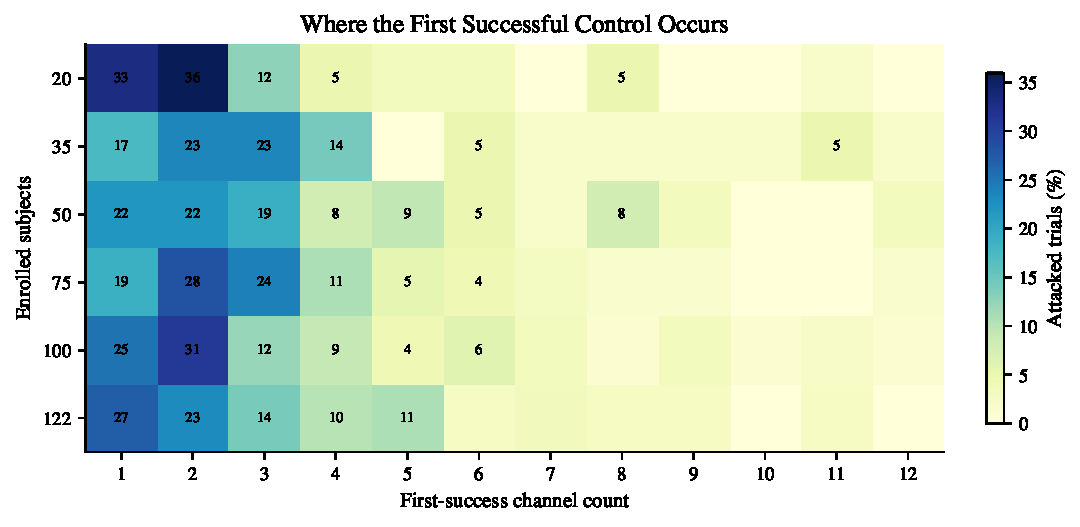
\includegraphics[width=0.78\textwidth]{Figure/hbn_first_success_heatmap.pdf}
}{%
  \fbox{\parbox{0.8\textwidth}{Figure/hbn_first_success_heatmap.pdf not found.}}
}
\end{center}
\vspace{-0.3em}
\begin{center}
\small The mass is concentrated around one to three channels, with a smaller tail of harder trials.
\end{center}
\end{frame}

% ------------------------------------------------------------
\begin{frame}{Why These Results Make Sense}
\begin{enumerate}
  \item Adding more identities makes clean recognition harder, so accuracy drops and EER rises.
  \item A non-targeted attack only needs to cross the nearest decision boundary.
  \item Some electrode traces carry high leverage for the current subject decision.
  \item SCS searches for those traces and changes them using EEG-band waveforms.
  \item This explains why high ASR can coexist with low \(k^\star\).
\end{enumerate}

\smallgap
\begin{center}
\small This is an interpretation of the observed behavior, not a universal scaling law.
\end{center}
\end{frame}

% ------------------------------------------------------------
\begin{frame}{Why Complete-Channel Control Matters}
\begin{table}
\centering
\footnotesize
\begin{tabular}{p{0.34\textwidth}p{0.34\textwidth}cc}
\toprule
Variant & Perturbation model & ASR & Mean \(k^\star\)\\
\midrule
SCS & Score-only complete-channel waveform search & 72.66\% & 3.47\\
SAGA-style sparse channel-time PGD & Gradient-based sparse channel-time samples & 9.38\% & 4.92\\
Sparse channel-time + hybrid waveform & Score-only channel-time ablation & 13.28\% & 4.88\\
\bottomrule
\end{tabular}
\end{table}

\begin{center}
\small BNCI2014\_001 reference comparison: controlling complete electrode traces is much more effective in this setting than sparse channel-time changes.
\end{center}
\end{frame}

% ------------------------------------------------------------
\begin{frame}{Limitations To Say Clearly}
\begin{itemize}
  \item This is a digital attack evaluation, not hardware-in-the-loop signal injection.
  \item SCS is a heuristic; failure within budget does not certify robustness.
  \item The HBN scaling study uses one release and six nested subject counts.
  \item The results support a persistence claim from 20 to 122 subjects, not a universal law for all EEG tasks.
  \item All HBN attacks use a fixed query cap; a full query-efficiency curve is future work.
\end{itemize}
\end{frame}

% ------------------------------------------------------------
\begin{frame}{Final Takeaways}
\begin{enumerate}
  \item The work studies a realistic score-only question: can output scores alone guide an EEG attack?
  \item The sparse unit is a complete electrode trace because that matches the EEG acquisition interface.
  \item The waveform basis keeps perturbations in EEG-relevant frequency structure.
  \item SCS solves the hard problem by separating channel selection from waveform refinement.
  \item \(k^\star\) turns attack success into a channel-level security measurement.
  \item On HBN, SCS remains high-success and low-channel from 20 to 122 enrolled subjects.
\end{enumerate}

\smallgap
\begin{center}
\alert{Short version: find high-leverage channels, inject small EEG-band waveforms, and measure how many channels are enough to flip the decision.}
\end{center}
\end{frame}

\end{document}
